% !TeX root = ../main.tex

\chapter{Introduction}

\begin{figure}[!t]
    \centering
    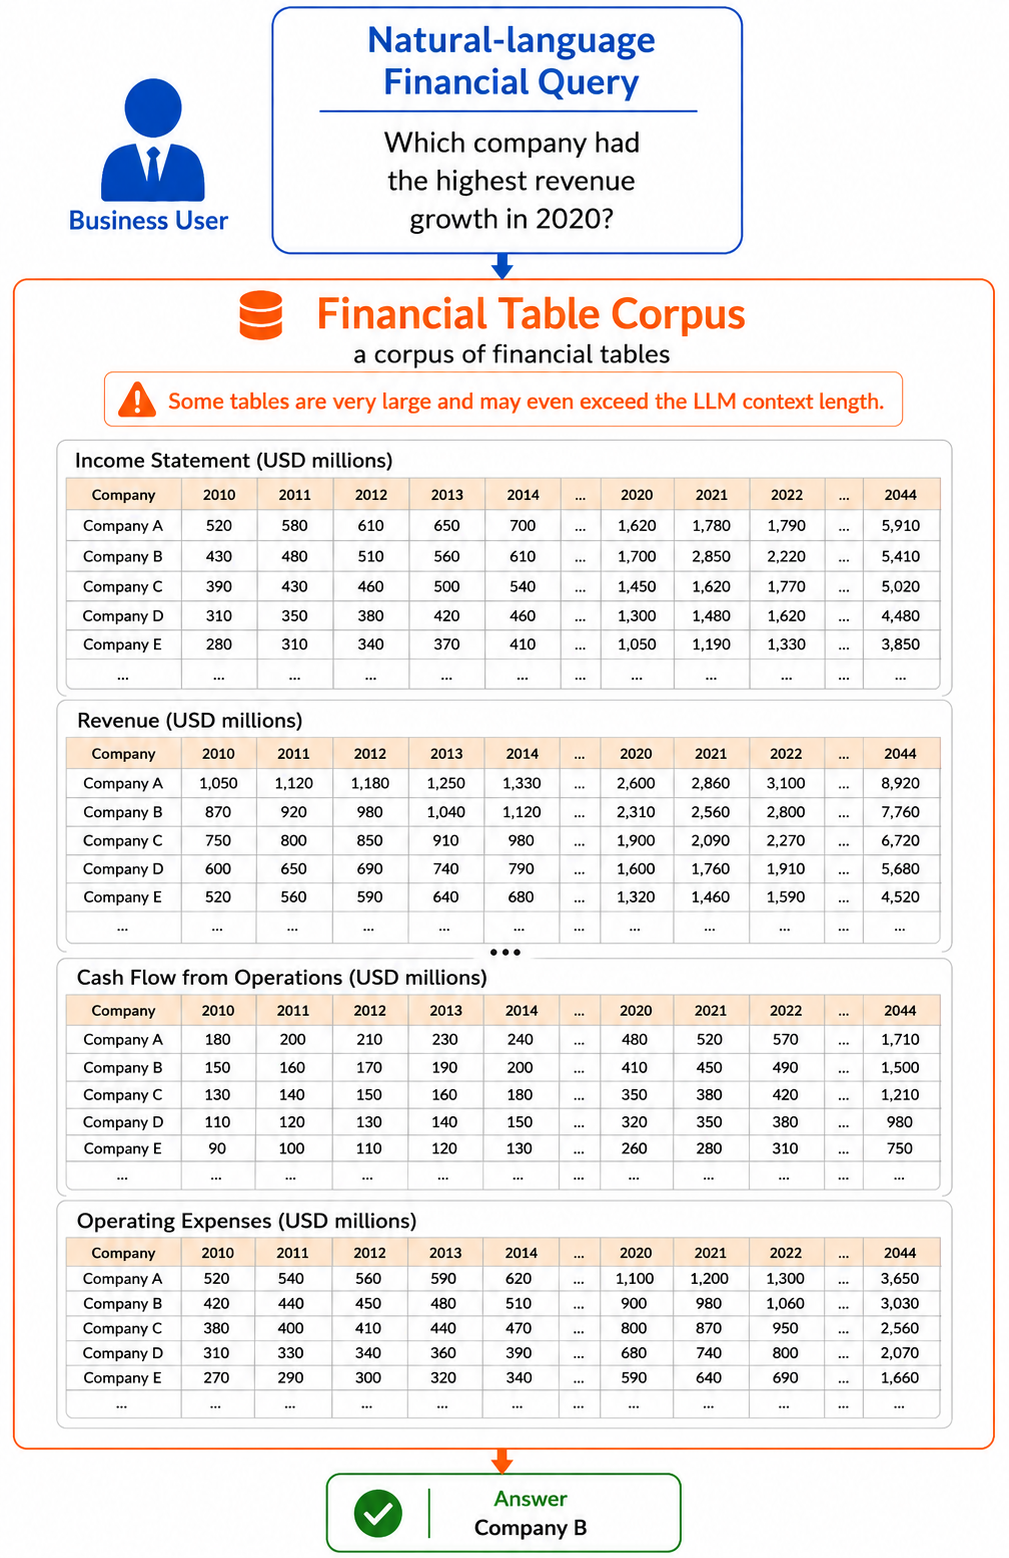
\includegraphics[width=\columnwidth]{figures/financial_example.png}
    \caption{Open-domain large table question answering in financial applications. A user asks a natural-language question over a corpus of financial tables and expects the system to identify the relevant information and produce the answer. Individual tables can be very large and may even exceed the LLM context limit.}
    \label{fig:financial_motivation}
\end{figure}

In real-world financial and business applications, users frequently query over numerous large tables.
For example, the London Stock Exchange Group~\cite{lseg_products} provides frequently accessed APIs for databases containing thousands of tables, which describe various companies and their financial indicators spanning multiple years.
Yet, ordinary users often know neither which table contains the required information nor how to formulate an executable query.
Instead, they prefer to query the data directly in natural language.
Figure~\ref{fig:financial_motivation} illustrates such a setting, where a user asks a natural-language financial question and expects an answer extracted from a corpus of financial tables.

Open-Domain Table Question Answering (OTQA) systems answer natural language questions over a corpus of tables. 
A typical OTQA pipeline consists of two stages: table retrieval and table reasoning.
The retrieval stage identifies candidate tables from the corpus, which are subsequently used by the reasoning stage to produce the final answer.

However, existing OTQA methods are primarily studied on relatively small tables and may not scale effectively to large tables.
During table retrieval, full-content table representations may incorporate substantial query-irrelevant cell-level information, diluting query-relevant semantic signals and potentially reducing retrieval effectiveness.
During table reasoning, large tables may be impractical to provide in full to the LLM, requiring the table information to be reduced before reasoning. However, the resulting table context may omit information required to answer the query, degrading reasoning quality and ultimately reducing end-to-end QA accuracy.

To study the challenges introduced by large tables, we focus on Open-Domain Large-Table Question Answering (OLTQA).
OLTQA extends the standard OTQA setting to a corpus containing large tables, where individual tables can exceed the context window of state-of-the-art LLMs when fully serialized for reasoning.

To systematically study OLTQA, we conduct experiments on a public benchmark.
We derive an OLTQA dataset from the closed-domain DataBench benchmark for open-domain evaluation.
DataBench contains substantially larger tables than existing OTQA benchmarks, making it suitable for examining the effect of table scale.


To address the challenges of OLTQA over large tables, we propose a practical approach.
Our approach combines schema-level table representations for table retrieval with interactive multi-table reasoning.
For table retrieval, schema-level representations avoid incorporating excessive cell content.
For table reasoning, building on TableRAG~\cite{tablerag}, we use schema and cell retrieval to construct a compact table context, avoiding the need to provide the full large table to the reasoner.
When the resulting context omits necessary information, interactive table access allows the reasoner to obtain additional table information during reasoning.
To reduce dependence on the top-ranked retrieval result, the reasoner operates over multiple retrieved candidate tables rather than relying solely on the top-ranked table.
Experimental results demonstrate that our proposed pipeline consistently outperforms existing OTQA baselines across all evaluated LLM backbones.

We further evaluate OLTQA in a real-world financial corpus.
Unlike DataBench, the financial corpus consists of hundreds of tables from the same domain and is maintained in a continuously updated database. The real-world financial setting introduces practical constraints on content-dependent offline preprocessing and makes table discrimination particularly challenging when multiple tables share similar schemas.
The financial-corpus evaluation complements DataBench by examining OLTQA under practical constraints and domain-specific ambiguity.

Through closed-domain experiments and qualitative error analysis, we further examine reasoning stage performance, identify major failure modes in current OLTQA pipelines, and characterize directions for future improvement.

Our contributions are summarized as follows:
\begin{itemize}
\item We explicitly define the OLTQA research setting and systematically study table retrieval and reasoning over large individual tables. 
\item  We derive an OLTQA dataset from DataBench for open-domain evaluation and conduct extensive experiments across multiple LLM backbones and table scales.
\item We develop a practical approach that substantially outperforms existing baselines while maintaining competitive input-token usage.
\item We further conduct evaluations on a real-world financial table corpus, revealing practical challenges not fully captured by public benchmarks.
\item We conduct comprehensive qualitative error analysis to identify the major failure modes of current systems and derive directions for future improvement. 
\end{itemize}
